\chapter{Related Work}
\label{relatedwork}
There has been a lot of research in the field of Virtual Reality and manipulating a virtual environment, most recent summarized by Jankowski in 2015. \cite{interactions:Jankowski2015} Further reading about specific techniques and tools can be found in Section \ref{theory:toolsandtech}. There have been a number of studies and implementations of systems that manipulates 3D environments using a HMD. The first major stride within this was in a study Butterworth in 1992 where a 3D surface modeling program was developed. \cite{relatedwork:Butterworth1992} This system was created using the same principles as CAD \footnote{http://www.autodesk.com/solutions/3d-cad-software} and similar software withing 3D object creation and manipulation. Since then there has been numerous other studies and applications withing 3D object creation with a HMD \cite{relatedwork:bowman1996conceptual} \cite{relatedwork:moshell1995research} \cite{relatedwork:liang1994jdcad}

Aswell as for the objects themselves, there has been soem studies about using a HMD to manipulate 3D objects in relation to a virtual environment. This approach is not as focused on 3D modelling as much as postitioning and scaling of pre-fabricated objects in a 3D environment. In a study by Stoakley in 1995 a system called World in Miniature (WIM) was created.\cite{relatedwork:stoakley1995virtual} The premis of this system is to display a miniature version of the virtual environment aswell as the full-scale one. This allows the user to perform delicate manipulations at full scale, and bigger more fundamental changes on the miniature version. The user is holding a clipboard in one hand which represents the miniature world, and a interactive ball in the other for selecting and manipulating in 3D space. The same year, Mine introduced the "Immersive Simulation
Animation And Construction" system (ISAAC).\cite{relatedwork:mine1995isaac} This system is primarly for designed for scene composition and interactive contstruction of virtual worlds. It tries to take advantage of the possibilities in the virtual world but keep the interaction scheme similar to the real world for easier adaptaion to less experienced users. ISAAC uses multiple types of tools for object manipulation, such as ray-cast and direct manipulation (see Section \ref{theory:toolsandtech}) and multiple tools for the user to travel. This system is more of a showcase then a real-world applicaton, as it demonstrates many of the posibilities with object and scene manipulation with a HMD but does not limit interaction tools or a specific purpose.

There have been some studies about merging a regular workstation for 3D manipulation with a HMD. One of these which had a purpose similar to the objective of this thesis has been researched and developed by Bowman et al. back in 1997. \cite{relatedwork:kijimaand1997transition} The authors investigated how to combine a regular work setup for 3D development with a HMD to remove the repeated transition between the two. Their Augmented Reality (AR) system is based on a real workstation which consists of a computer together with screen, keyboard and mouse. This is combined with a Projective Head Display (PHMD) to create an environment where the user can see projected 3D objects and still be able to use the workstation as usual.
\section{Applications}
Since the release of both the Oculus rift \footnote{https://www.oculus.com/rift/} and HTC Vive \footnote{https://www.vive.com/eu/product/} which both have 6 DOF controllers, the number of applications focusing on complex interactions and manipulation has really exploded.
\subsection{Storyboard VR}
The creative team at Artefact \footnote{https://www.artefactgroup.com/} created a prototyping tool for VR called Storyboard VR \footnote{https://www.artefactgroup.com/work/storyboard-vr/}. This tool gives the user the option to create high fidelity(see section \ref{method:prototype:hifi})  VR prototypes while immerged with a HMD. Objects in the scene are uploaded as high-resolution images and placed in the virtual environment. The essential interactions of this system are listed below
\subsubsection{Tools}
To interact with this system the primary controller is equipped with a ray-casting technique (see section \ref{theory:toolsandtech:raycast}) for selection within the virtual environment.
Most tools in this system can be found on a swipe-based menu, attached to the secondary controller. There are some object-specific selectors (see section \ref{theory:toolsandtech:selector}) attached to each object, these are visible when the object is selected by the user. It is not possible to teleport or in other ways travel in the application, but there are  a timeline/storyline where different 'frames' can be accessed.

\subsubsection{Creating objects}
In order to create an object within the world, the user can select from imported images or default 3D shapes from the 'Create' part of the menu. An object that has been created can later be duplicated by selecting 'Duplicate' on the same menu and then selecting the object.
\subsubsection{Selecting and deleting objects}
Objects are selected by pointing the ray from the primary controller on the and clicking the trigger. An object is deleted by selecting the object and selecting remove on the menu.
\subsubsection{Scale and positioning}
Changing the position of an object is achieved by pointing the ray at the object, holding the trigger while moving it into position with the ray, then releasing the trigger. The scale of an object is manipulated by using the touchpad on top of the primary controller.
\subsection{Tilt Brush}
\label{relatedwork:tiltbrush}
 One of the most known application is 'Tilt Brush' \footnote{https://www.tiltbrush.com/} for HTC Vive where the user can use the existing handcontrollers as paintbrushes and paint in 3D space. This application highlights many of the interactions that are essential when manipulating a the environment. Some of these are listed below:
\subsubsection{Creating objects}
Creating an object or in this case a new painting stroke is the core of the application, and can as such be accessed directly with primary triggers on both controllers.
\subsubsection{Selecting and deleting objects}
Objects (strokes) are targeted by placing a spherical tool (attached to your brush) around the stroke and pressing the same trigger that is used for drawing. The tool is activated by selection on the secondary brush menu.
\subsubsection{Parameters and setting}
The most common and used tools for what will be painted ( brush-size, undo, deleting strokes etc) are accessed through the primary brush (controller). More complex modifications (brush type, colors etc) are accessed from the secondary brush by activating a menu connected to that brush (controller) and selecting with the other brush.
\begin{figure}
\begin{subfigure}{.5\textwidth}
  \centering
  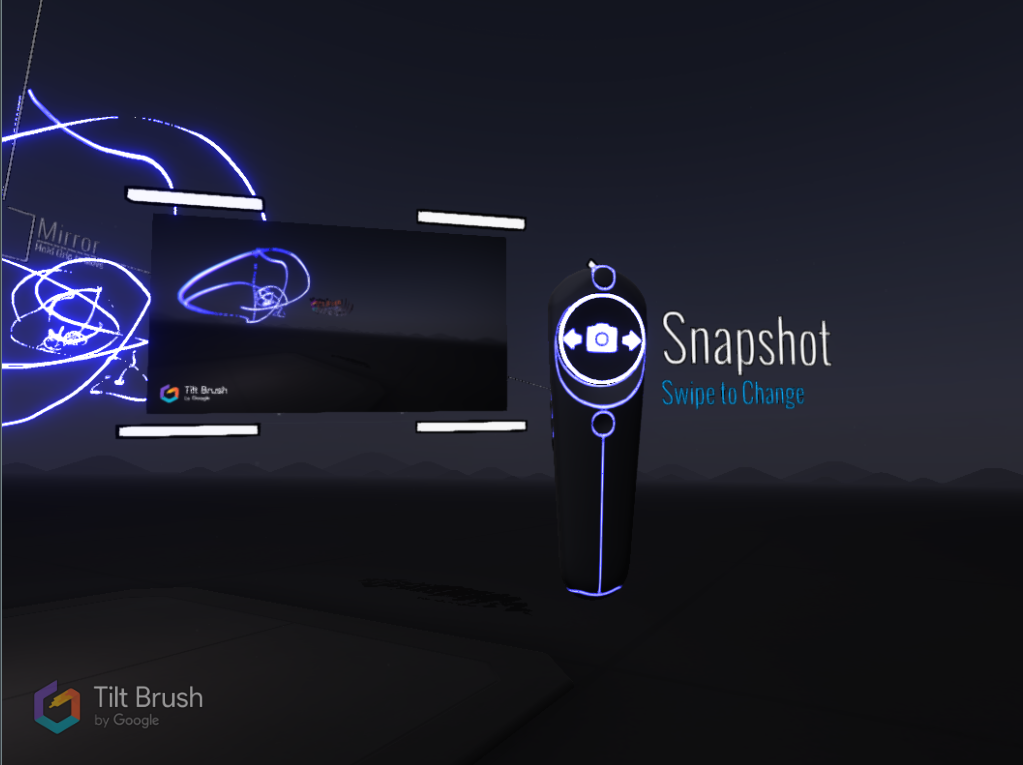
\includegraphics[width=.8\linewidth]{tilt_activemenu.PNG}
  \caption{Active menu. Selection of mode depending on current tool}
  \label{fig:sfig1:tilt_activemenu}
\end{subfigure}%
\begin{subfigure}{.5\textwidth}
  \centering
  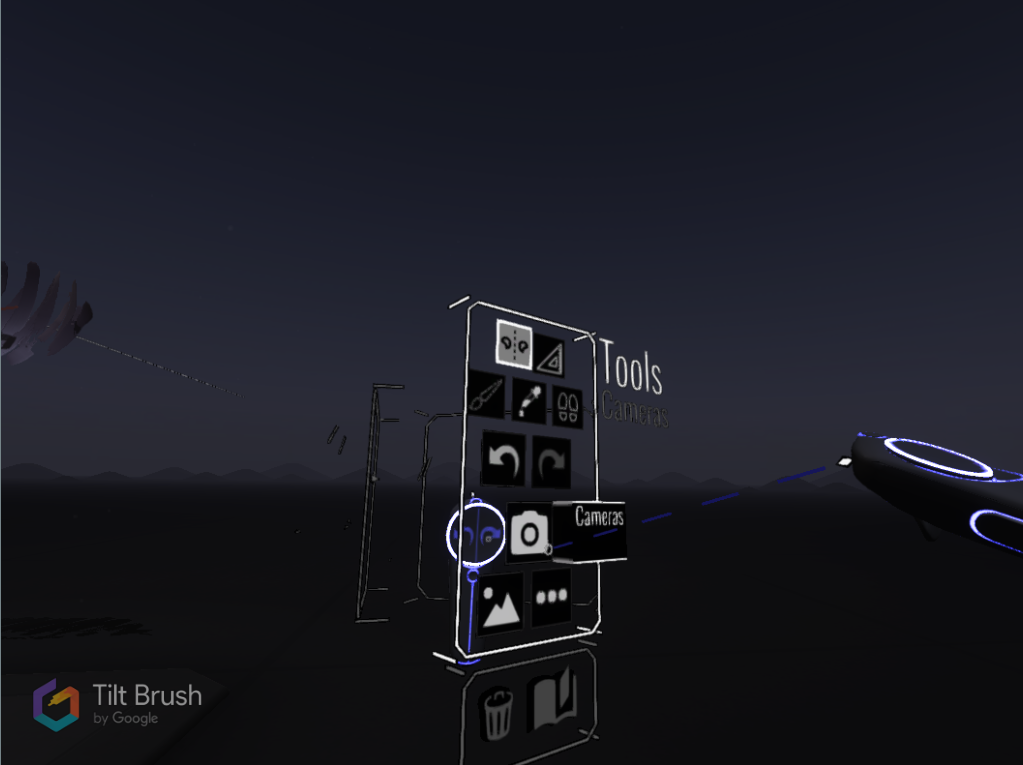
\includegraphics[width=.8\linewidth]{tilt_passivemenu.PNG}
  \caption{Passive menu with all actions and tools. Always avaliable in secondary hand. }
  \label{fig:sfig2:tilt_activemenu}
\end{subfigure}
\caption{Menu interfaces in Tilt Brush}
\label{fig:fig:tilt_menu}
\end{figure}
\subsection{Scale and positioning}
One of the biggest advantages of working in a virtual environment is that you are not bound to the restrictions of your physical relatioonship to the objects that you are working with. By using both controllers and moving them away from eachother, the environment grows and the users scale decreases. The user scale can be enlarged by moving the controllers closer together.
By using a raycast (see Section \ref{theory:toolsandtech}) the user can teleport around in the virtual environment.
